\section{Architecture}
There system consists of four components, which are all defined in their own packages. Figure \ref{fig:img-architecture} illustrates how the components are connected together.

\FloatBarrier
\begin{figure}
\centering
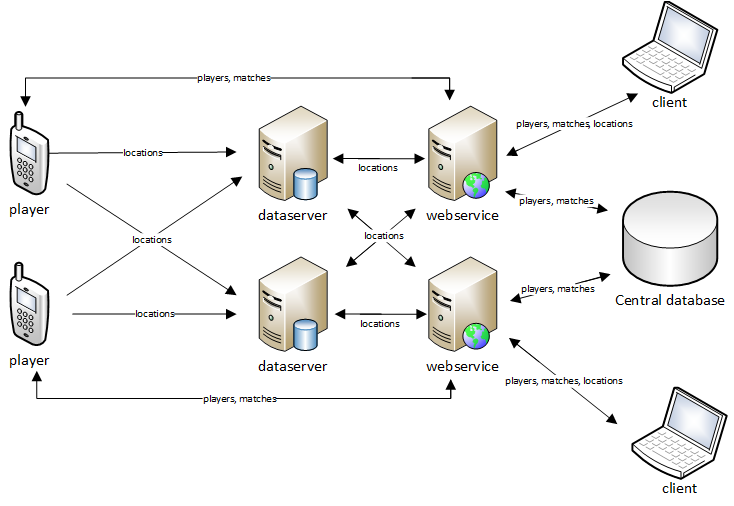
\includegraphics[scale=0.7]{img/architecture.png}
\caption{An overview of the architecture.}
\label{fig:img-architecture}
\end{figure}

\begin{description}
\item[Player] \hfill \\
Players represent the sports(wo)men who have their location monitored during a match. In an ideal world, they would carry devices that send the location periodically to a server. We simulated this by creating an Android app that has the following functionalities:
\begin{itemize}
    \item The user can select who he is, by providing a list of known players on the Webservice.
    \item The app shows a list of available matches, fetched from the Webservice, which show the match details. The user can click on a match to go to the detail view.
    \item When the user is in a match detail view, monitoring can be started. This will send the location of the player periodically to a DataServer provided by the match details.
\end{itemize}
\item[DataServer] \hfill \\
DataServers do two things. First of all, they listen for incoming location packets and store them in their local database. Secondly, they listen for requests, made by Clients (through the Webservice) for all locations, for a given player and match, and respond by sending the locations to the callback provided in the request.
\item[Webservice] \hfill \\
The Webservice provides endpoints for both Players and Clients to communicate to. It also has a connection with all DataServers to request locations when a Client asks for it. The functionalities which are implemented:
\begin{itemize}
    \item Serves lists of all players and matches, retrieved from a central database and used by Clients and Players.
    \item Endpoints for creating new players and matches, which are consequently stored in a central database. These endpoints are used by Clients.
    \item Endpoint for Clients to request all locations for a given match and player. When such a request is received, the Webservice asks all DataServers if they have locations for this match/player. The Webservice sends the received locations back to the Client.
\end{itemize}

\item[Client] \hfill \\
The Client is mainly used by coaches and offers the following functionalities:
\begin{itemize}
    \item Create new matches and players by providing forms and sending the input to the Webservice.
    \item Request all locations for a given match and player, by showing a list of all matches and players in the Webservice, which the client can select. The locations are requested from the Webservice (which in turn communicates with the DataServers).
\end{itemize}
\end{description}